%% LyX 1.5.5 created this file.  For more info, see http://www.lyx.org/.
%% Do not edit unless you really know what you are doing.
\documentclass[a4paper,czech,czech,openright,cleardoubleempty,BCOR10mm,DIV11]{scrreprt}
\usepackage[T1]{fontenc}
\usepackage[utf8]{inputenc}
\usepackage{array}
\usepackage{longtable}
\usepackage{varioref}
\usepackage{wrapfig}
\usepackage{fancybox}
\usepackage{calc}
\usepackage{framed}
\usepackage{url}
\usepackage{graphicx}
\usepackage{placeins} %floatbarrier \FloatBarrier
%\usepackage{listing}
\usepackage{pdfpages}

\makeatletter

\usepackage[font=small,labelfont=bf]{caption} %captiony

%%%%%%%%%%%%%%%%%%%%%%%%%%%%%% LyX specific LaTeX coěmmands.
\providecommand{\LyX}{L\kern-.1667em\lower.25em\hbox{Y}\kern-.125emX\@}
\newcommand{\lyxline}[1][1pt]{%
  \par\noindent%
  \rule[.5ex]{\linewidth}{#1}\par}
\newcommand{\noun}[1]{\textsc{#1}}
%% Special footnote code from the package 'stblftnt.sty'
%% Author: Robin Fairbairns -- Last revised Dec 13 1996
\let\SF@@footnote\footnote
\def\footnote{\ifx\protect\@typeset@protect
    \expandafter\SF@@footnote
  \else
    \expandafter\SF@gobble@opt
  \fi
}

\renewcommand{\baselinestretch}{1.2} %radkovani s

\expandafter\def\csname SF@gobble@opt \endcsname{\@ifnextchar[%]
  \SF@gobble@twobracket
  \@gobble
}
\edef\SF@gobble@opt{\noexpand\protect
  \expandafter\noexpand\csname SF@gobble@opt \endcsname}
\def\SF@gobble@twobracket[#1]#2{}
%% Because html converters don't know tabularnewline
\providecommand{\tabularnewline}{\\}

%%%%%%%%%%%%%%%%%%%%%%%%%%%%%% Textclass specific LaTeX commands.
\newenvironment{lyxcode}
{\begin{list}{}{
\setlength{\rightmargin}{\leftmargin}
\setlength{\listparindent}{0pt}% needed for AMS classes
\raggedright
\setlength{\itemsep}{0pt}
\setlength{\parsep}{0pt}
\normalfont\ttfamily}%
 \item[]}
{\end{list}}

%%%%%%%%%%%%%%%%%%%%%%%%%%%%%% User specified LaTeX commands.
%<-------------------------------společná nastavení------------------------------>
\usepackage[czech]{babel}%počeštění názvů (Obsah, Kapitola, Literatura atp.)
\usepackage[]{hyperref} %odkazy v  pdf jsou klikací s barevnými rámečky
\usepackage[numbers,sort&compress]{natbib} %balíček pro citace literatury  
\usepackage{hypernat}%interakce mezi hyperref a natbib
\newcommand{\BibTeX}{{\sc Bib}\TeX}%BibTeX logo
\hypersetup
{   % Nastavení polí PDF dokumentu 
pdftitle={IT pro podporu seniorů v domácím prostředí},%   
pdfauthor={Petr Scholz},%  
pdfsubject={},%   
pdfkeywords={IT, AI, AAL}%                             
}
\usepackage{multicol}




%<-----------------------------volání stylů----------------------------------------->
% (znak % je označení komentáře: co je za ním, není aktivní)
%<------------------------------------písmo----------------------------------------->
%\usepackage{packages/bc-latinmodern}
%\usepackage{packages/bc-times}
\usepackage{packages/bc-palatino}
%\usepackage{packages/bc-iwona}
%\usepackage{packages/bc-helvetika}


%<------------------------------záhlaví stránek------------------------------------>
%\usepackage{packages/bc-headings}
\usepackage{packages/bc-fancyhdr}

%<------------------------------hlavičky kapitol------------------------------------>
%\usepackage{packages/bc-neueskapitel}
%\usepackage{packages/bc-fancychap}

\makeatother

\usepackage{babel}

%java code block%

\usepackage{listing}
\usepackage{listings}
\usepackage{color}

\definecolor{dkgreen}{rgb}{0,0.6,0}
\definecolor{gray}{rgb}{0.5,0.5,0.5}
\definecolor{mauve}{rgb}{0.58,0,0.82}

\renewcommand*{\lstlistingname}{Ukázka kódu} %prejmenovani 
\renewcommand*{\lstlistlistingname}{Seznam ukázek kódu}

% syntax highlight pro jazyk Java %
\lstset{
  %frame=r,
  captionpos=b,
  language=Java,
  aboveskip=3mm,
  belowskip=3mm,
  xleftmargin=0.2mm,
  showstringspaces=false,
  columns=flexible,
  basicstyle={\small\ttfamily},
  numbers=none,
  numberstyle=\tiny\color{gray},
  keywordstyle=\color{blue},
  commentstyle=\color{dkgreen},
  stringstyle=\color{mauve},
  breaklines=true,
  breakatwhitespace=true,
  tabsize=3,
    inputencoding=utf8,
    extendedchars=true,
    literate=%
    {á}{{\'a}}1
    {č}{{\v{c}}}1
    {ď}{{\v{d}}}1
    {é}{{\'e}}1
    {ě}{{\v{e}}}1
    {í}{{\'i}}1
    {ň}{{\v{n}}}1
    {ó}{{\'o}}1
    {ř}{{\v{r}}}1
    {š}{{\v{s}}}1
    {ť}{{\v{t}}}1
    {ú}{{\'u}}1
    {ů}{{\r{u}}}1
    {ý}{{\'y}}1
    {ž}{{\v{z}}}1
    {Á}{{\'A}}1
    {Č}{{\v{C}}}1
    {Ď}{{\v{D}}}1
    {É}{{\'E}}1
    {Ě}{{\v{E}}}1
    {Í}{{\'I}}1
    {Ň}{{\v{N}}}1
    {Ó}{{\'O}}1
    {Ř}{{\v{R}}}1
    {Š}{{\v{S}}}1
    {Ť}{{\v{T}}}1
    {Ú}{{\'U}}1
    {Ů}{{\r{U}}}1
    {Ý}{{\'Y}}1
    {Ž}{{\v{Z}}}1
}

\begin{document}
%~\thispagestyle{empty}{\small ~\vfill{}
%}{\small \par}

%~\thispagestyle{empty}\vfill{}
%Tato stránka je tzv. protititul a je graficky součástí titulní stránky.
%Nechte ji prázdnou, nebo na ni umístěte vhodnou fotografii či ilustraci.

\cleardoublepage{}~\thispagestyle{empty}\begin{center}\pagenumbering{roman}\vspace{10mm}


\textsf{\textsc{\noun{\LARGE Univerzita Hradec Králové}}}\\
\vspace{0.5em}
\textsc{\noun{\LARGE Fakulta informatiky a managementu}}\\
\vspace*{1em}
\textsf{\textsc{\noun{\Large katedra informačních technologií }}}

\vspace{15mm}

%
\includegraphics[width=0.4\textwidth]{logo/uhk}

\vspace{15mm}


\textsf{\huge BAKALÁŘSKÁ PRÁCE}{\huge \par}

\vspace{15mm}


\textsf{\LARGE IT pro podporu seniorů v domácím prostředí}{\LARGE \par}

\vspace{10mm}


\end{center} 

\vspace*{\fill}


\vspace{10mm}


\begin{description}
\item [{{\large Autor:}}] \noindent \textsf{\large Petr Scholz}{\large \par}
\item [{{\large Vedoucí~práce:}}] \noindent \textsf{\large prof. RNDr. Peter Mikulecký, PhD.}{\large \hfill{}}\textsf{\large Hradec Králové, 2014}{\large{}
% doplňte rok vzniku vaší bakalářské práce
}{\large \par}
\end{description}
\clearpage{}

%{\small \thispagestyle{plain}\addcontentsline{toc}{chapter}{Abstrakt} }{\small \par}

\newpage{}\thispagestyle{plain}

{\small %\setcounter{page}{3} % nastavení číslování stránek
\ }{\small \par}

\noindent {\small \vfill{}
 % nastavuje dynamické umístění následujícího textu do spodní části stránky
~}{\small \par}

\subsubsection{Prohlášení}

\noindent {\small 

Prohlašuji, že svou bakalářskou práci “IT pro podporu seniorů v domácím prostředí“ jsem vypracoval samostatně pod vedením vedoucího bakalářské práce a s použitím odborné literatury a dalších informačních zdrojů, které jsou citovány v práci a uvedeny v seznamu literatury.

}{\small \par}

{\small \bigskip{}
}\noindent {\small{} V Hradci Králové dne \today\hspace{\fill}Michael Kutý}\\
{\small{} % doplňte patřičné datum, jméno a příjmení
}{\small \par}

\clearpage{}

\newpage{}\thispagestyle{plain}

{\small %\setcounter{page}{3} % nastavení číslování stránek
\ }{\small \par}

\noindent {\small \vfill{}
 % nastavuje dynamické umístění následujícího textu do spodní části stránky
~}{\small \par}

\subsubsection{Poděkování}

\noindent {\small 

Děkuji prof. RNDr. Peter Mikulecký, PhD. za odborné vedení práce a poskytování cenných rad. Dále bych chtěl poděkovat všem seniorům, kteří si našli čas na vyplnění mého dotazníku.

 \newpage{}}{\small \par}

\clearpage{}

\newpage{}\thispagestyle{plain}

{\small %\setcounter{page}{3} % nastavení číslování stránek
\ }{\small \par}

\noindent {\small \vfill{}
 % nastavuje dynamické umístění následujícího textu do spodní části stránky
~}{\small \par}

\subsubsection{Anotace}

Tato bakalářská práce je věnována tématu ambientní inteligence a skládá se ze tří částí. První část je teoretická, ve které jsou použity poznatky z odborné literatury a článků. Druhá část je založena …

\subsubsection{Annotation}

This thesis is devoted to ambient inteligent and consist of two parts. The first part is theoretical, where findings from the literature are used. The sekond part is based on….

\cleardoublepage{}

%\thispagestyle{empty}~{\small \addcontentsline{toc}{chapter}{Zadání
%práce} }{\small \par}

{\small %%%   Výtisk pak na tomto míste nezapomeňte PODEPSAT!
%%%                                         *********
}{\small \par}

\cleardoublepage{}\thispagestyle{empty}{\small 
%\setcounter{secnumdepth}{3}
%\setcounter{tocdepth}{2}%hloubla obsahu
\tableofcontents{}% vkládá automaticky generovaný obsah dokumentu
\cleardoublepage{}}{\small \par}


\include{uvod}

\include{cile_a_metodika_prace}

\include{analyza_problemu}

\include{navrh_reseni}

\include{experimentalni_implementace}

\include{vysledky_a_jejich_diskuze}


\chapter[Shrnutí výsledků]{Shrnutí výsledků}

Cílem této práce bylo seznámení s ambientní inteligencí... 

\chapter[Závěr]{Závěr}


Cílem této práce bylo seznámení s ambientní inteligencí... 

Cílem této práce bylo seznámení s ambientní inteligencí... 

\begin{thebibliography}{10}

%\bibitem{cmejrkova}ČMEJRKOVÁ, Světla, František DANEŠ a Jindra SVĚTLÁ \emph{Jak napsat odborný text.}
%{Vyd.1. Praha: Leda}, {ISBN 80-859-2769-1.} }


\end{thebibliography}

\addcontentsline{toc}{chapter}{Literatura} 

\cleardoublepage{}

%\include{prilohy}

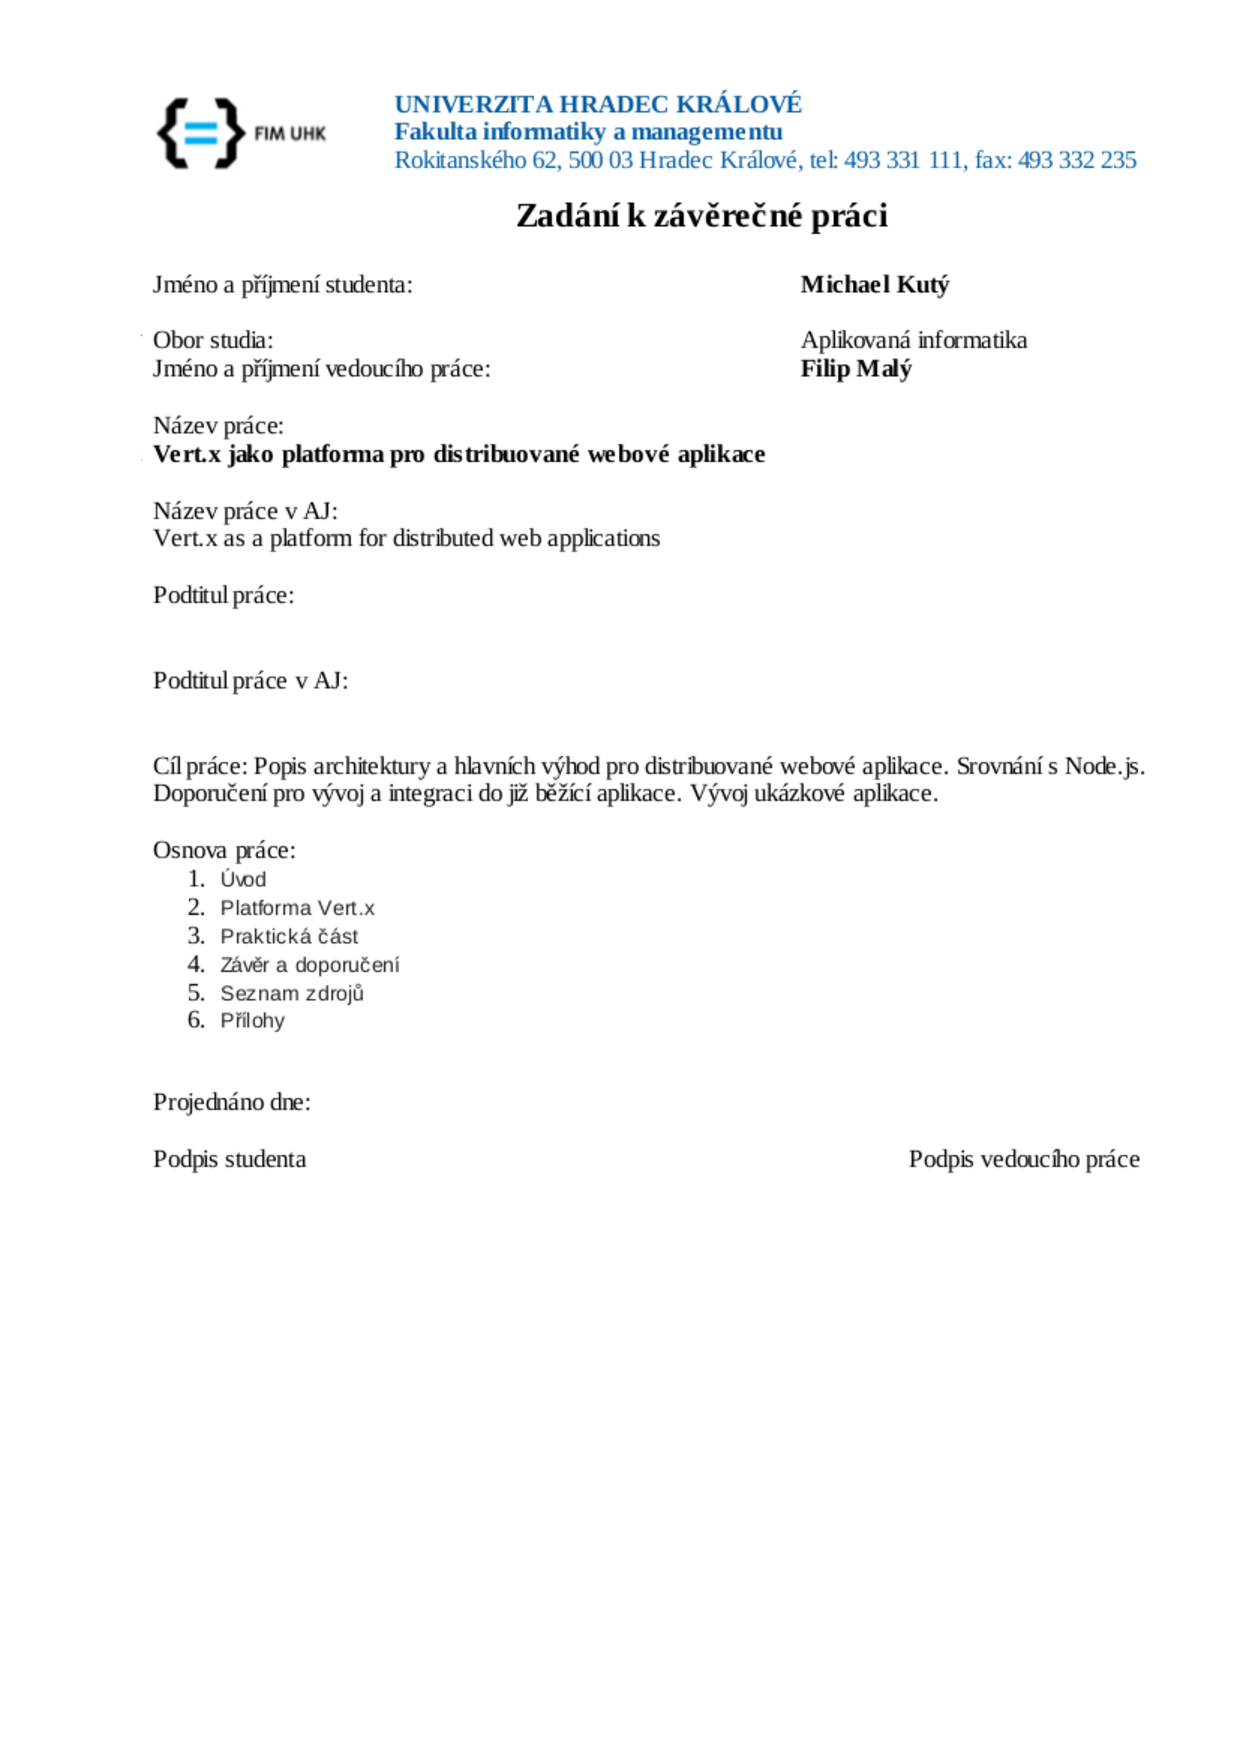
\includepdf[pages={1}]{zadani.pdf}

\end{document}
